\documentclass{article}
\usepackage{subfigure}
\usepackage{todonotes}
\usepackage{times,amsmath,epsfig}
%\title{Thesis\\ Responses to Reviewers' Comments}
\begin{document}
%\maketitle

\section*{Reply to Examiner No. 2}
\begin{table}[h]
	%	\centering
	%	\caption{Popular window-based FIR filter lengths}
	%	\label{tab:lengthFIR}
	%	\renewcommand{\arraystretch}{1.5}
	\begin{tabular}{ll}
		{\large From Candidate} &: {\large  Pham Hung Thinh} \\
		{\large Degree }& : {\large Doctor of Philosophy (PhD)}\\
		{\large Thesis Title }&: {\large Techniques for Multi-Standard Cognitive Radios on FPGAs}\\
		& \\
		& \\
		& 
	\end{tabular}
\end{table}




\begin{quote}
\emph{In terms of the dissertation topic, aspects of the physical implementation, digital signal processing techniques, and computation techniques are all highly relevant and timely. This is a technology that is ubiquitous worldwide, and broadly deployed in a number of commercial, private, and military domains. As Mr. Pham points out, this is not a ``one size fits all'' technology, and that different environmental and usage factors that influence the various standards. The work presented in this dissertation appeals to most use-cases where spectrum efficiency, computational efficiency, and link performance are primary factors.  }
	
\emph{Over the course of his PhD studies, Mr. Pham has generated several notable publications. While many remain under review, list of papers is impressive, and target highly relevant conferences and journals. While this work relates to cognitive radio applications, the decision making aspects of cognitive radio are not addressed in this dissertation, which is fine. Perhaps this should be made clear in the introduction.}
\end{quote}
First of all, thank you for your review. I have amended the text exactly as requested in the comments. This point has been added clearly in Chapter 1.

\begin{quote}
\emph{1. In Section 2.1, Mr. Pham states that OFDM system implementation is simple, low cost, and can be more effectively parameterized than FBMC systems. Further justification of this assertion is needed. It may be helpful to provide a more comprehensive comparison between OFDM and FBMC techniques.}
\end{quote}
This point has been amended in Section 2.1.1 to provide more comprehensive comparison between OFDM and FBMC described as follows:
In order to understand FBMC and its distinctness from OFDM, it is best to study multicarrier systems, in which the output signal can be expressed in the continuous time domain as Equ.\ref{equ:multicarriermodulation}.
This can be a unified formulation for both OFDM and FBMC.
\begin{eqnarray}
\label{equ:multicarriermodulation}
s(t) = \sum_{n}\sum_{k  = 0}^{N-1} x_{k}[n] h(t-nT)e^{i2\pi (t-nT)f_{k}},
\end{eqnarray}
where $x_{k}[n]$ denotes the sample of the $k_{th}$ subcarrier data symbol in $n_{th}$ symbol of continuous multicarrier symbols, $f_{k}$ is the $k_{th}$ subcarrier in a set of $N$ used subcarriers, $T$ is the multicarrier symbol duration, and $h(t)$ is a prototype filter.
\begin{figure}[b]
	\centerline{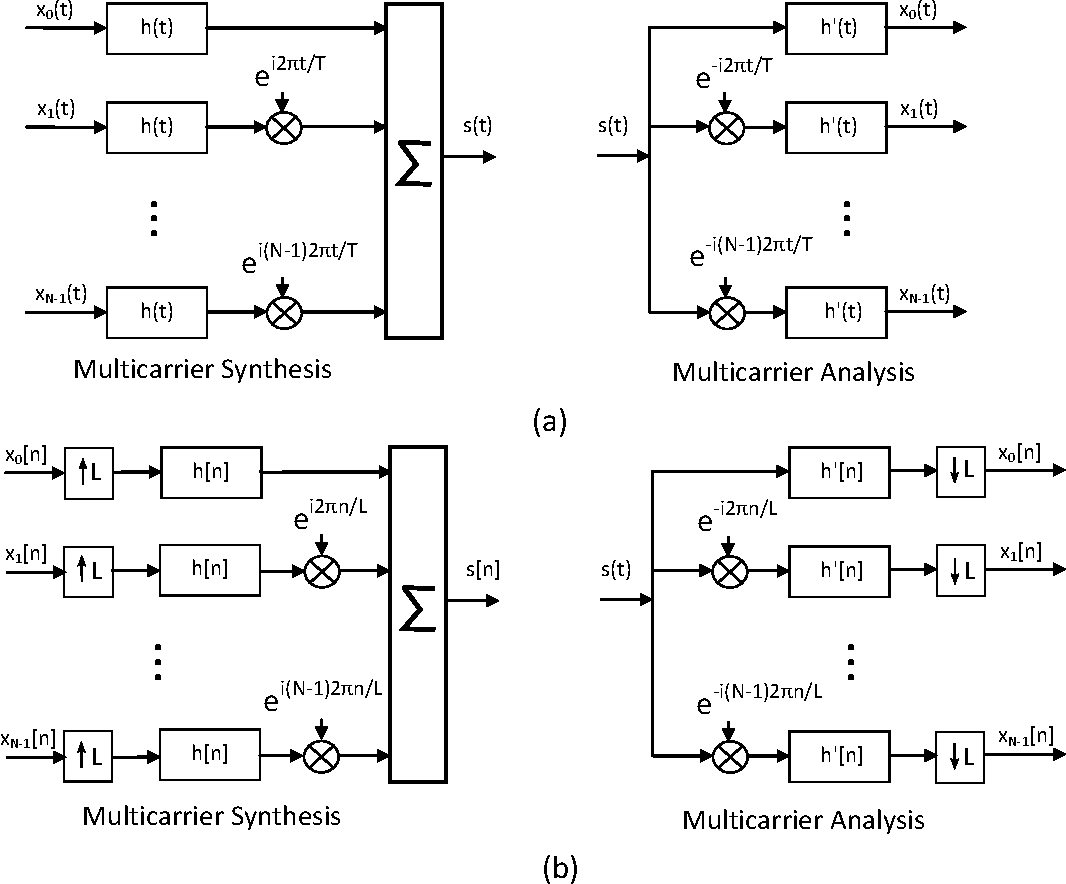
\includegraphics [width=0.8\columnwidth] {../Figures/multucarrier_system} }
	\caption{Block diagram of a multicarrier modulated system, (a) in the countinuous-time and (b) in discrete-time}
	\label{fig:multicarrier-block}
\end{figure}
This transceiver of multicarrier system can be modelled as a block diagram, shown in Figure~\ref{fig:multicarrier-block}.
As can be seen in the discrete-time domain, $N$ data symbols at synthesis are up sampled by a factor of $L$, which is calculated by $\frac{T}{T_{S}}$, $T_{S}$ denotes sample period of output sequence $s[n]$, and then filtered by a prototype filter $h[n]$. The output of each data stream will be modulated by frequency of multi-carriers and the summed for transmission.
The signal in the receiver is demodulated and then filtered by a bank of matched filters $h'[n]$, and down sampled by a factor of $L$.
When critical sampling applies, $L = N$ and the prototype filter $h[n]$ is selected as a rectangular pulse in the time domain, i.e. a $sinc$ pulse in the frequency, this multicarrier system becomes a conventional OFDM system.

FBMC is different from OFDM in the selection of the prototype filters $h[n]$, and matched filters $h'[n]$. Also, the $h[n]$ and $h'[n]$ filters are chosen and designed depending on the adopted FBMC modulation technique.
By using the well-designed filters for each subcarrier, FBMC could be a more effective solution in comparison to OFDM in term of ICI cancelation and spectral leakage suppression because nonadjacent subcarriers are almost completely separated by a bank of filters.

On the other hand, OFDM has been the dominant technique adopted for broadband multicarrier communication.
OFDM has many important and desirable features over the FBMC. OFDM was originally developed focusing on a low-complexity implementation. The low complexity of OFDM is achieved thanks to a fundamental assumption in which subcarriers of OFDM symbol are perfectly synchronized and orthogonal with the consecutive subcarriers. Thus the subcarriers are used for modulation at the transmitter using an IFFT block; inversely, they are separated by using an FFT block at the receiver. By contrast, FBMC may be more complex than OFDM. The demand for well-designed filters in FBMC results in increasing complexity and resource requirements. Moreover, while employing MIMO technique in OFDM to increase the system's capacity and resulting in high spectral efficiency is a straightforward work, unfortunately, the development of MIMO-FBMC systems is relatively more complex.
OFDM modulation has been the dominant technique adopted for many wireless standards and has been investigated in terms of spectral sensing and carrier allocation for CRs.
OFDM system implementation is simple, low cost, and can be more effectively parameterised.
A single baseband implementation can be made to flexibly support multiple standards like 802.11[14], 802.16[15], and 802.22[16], as well as supporting future OFDM-based standards.

\begin{quote}
\emph{2. Chapter 3 presents the multiplierless correlator work. There are aspects of this chapter that may need further examination. I appreciate the significance of the problem this chapter is addressing, and the value in the demonstrated savings; however, the methods for performing the comparisons don't always seem fair.
One note in resource usage: a DSP48 processing module is rated to operate at hundreds of MHz. If the desired operation speed is N times slower than the maximum operating speed, then a single DSP48 can cover N instances of the operation through time multiplexing. Therefore, when performing a resource estimate, the required number of units should be derated by the operational speed, otherwise it represents an underutilized system. In this case, the target operating frequency is 50 MHz while capacity of the DSP48s are over 300 MHz.	}
\end{quote}
The additional discussion on the aspect of operating speed is added as follows:
``The multiplierless correlator and the DSP-based correlator can operate at a speed which is multiple times higher than the desired operating speed for baseband modulation. Both of them can therefore make use of time multiplexing to obtain a trade-off between resource usage and operating speed. However, it should be noted that increased operating speed leads to significantly increased power since the power consumption is proportional to the square of operating frequency. To provide a fair comparison, both the multiplierless correlator and the DSP-based correlator are investigated on the same transposed direct form.''
The text in Section 3.2.3 has been amended to include this point.  But it should be noted that the structure of time multiplexing within the correlator is a potentially extensive research area in its own right, and is beyond the scope of the current investigation.


\begin{quote}
\emph{3. While power comparisons are made between the multiplierless version and DSP48 version, it isn't clear if the same highly quantized coefficients are being used in the DSP48 case. If not, I would expect those values to drop significantly. To a degree, this discussion breaks down into a traditional precision analysis problem. If indeed 32 bits of precision are not needed in this correlator, then the DSP48 could be the wrong component to use.}
\end{quote}
The use of a DSP48-based implementation when comparing to the multiplierless version is further discussed as follows:
``To obtain a precise computation, the DSP48 is typically used for multiplication in fixed point format, Q1.15. Because the DSP48 is a hard core, it is impossible to optimise the internal components of DSP48 in the case of reducing the number of bits used in the computation. The static power of the DSP based correlator will then not drop significantly when reducing the number of bits in the words being computed. Thus the use of DSP48 for calculation of words with fewer bits is wasteful as well as having reduced precision. Hence, it is not necessary to evaluate the DSP48 version employing just a small number of  bits for computation.''
This explanation is added in the chapter 3 at the Section 3.2.3.

\begin{quote}
\emph{4. It states that the multiplierless design must be specified manually, and cannot be inferred by the tools from higher level descriptions (I assume HDLs). After reviewing the structure presented in this chapter, I believe this assertion should be reexamnied.}
\end{quote}
This assertion has been revised to clarify the discussion as follows:
``The correlator designs must be specified manually, and cannot be inferred by the tools from higher level descriptions such as high level synthesis (HLS) or Simulink that allows designing systems at high level abstraction.''
This amendment is made in Section 3.2.

\begin{quote}
\emph{5. Taking advantage of the periodic nature of the energy distribution is an excellent way of reducing the computational burden of gross frame synchronization. When compared to full cross-correlation techniques this reduces the needed computation to a much smaller viable amount.}
\end{quote}
The computational reduction is further explained to show clearly how it achieves a significant decrease in terms of resource usage as follows:
``The proposed method improves upon full cross-correlation not just by taking advantage of the periodic nature of the preamble, but also profiting from the real number computation of the proposed metrics, instead of requiring complex computation, and through enabling the use of a multiplierless correlator, yielding a significant computational saving.''
This amendment is made in the chapter 4 at the subsection 4.3.4.2.

\begin{quote}
\emph{6. In Chapter 6, the performance of the proposed solution is very good, but seems to come at a significant computational cost due to the extension of the IFFT and increased sample rate. These costs should be quantified.}
\end{quote}
The discussion on computational cost is extended by providing a additional complexity analysis in terms of hardware usage (i.e. FFs and DSPs) for dynamically sized IFFT blocks and the FIR filter. This amendment is made in the chapter 6 at the subsection 6.4.2.

\begin{quote}
\emph{7. In Chapter 7, the premise is that faster reconfiguration is better, yet very little is provided on the requirements for when it is fast enough. There is significant emphasis on buffering streams at the boundaries of PR modules. I can appreciate the object of not wanting drop any data; however, for the radio standards discussed in previous chapters, there are higher-level protocols that manage the retransmission of lost or dropped packet of data.}
\end{quote}
I accept your point that higher layers can potentially handle the lost data, however it is good practice to prevent, or at least minimise, data loss in lower layers -- this is because of the tendency for lower-layer data loss to have more serious knock-on effects at higher layers (i.e. the  loss magnification when climbing the layer stack). This point is now discussed in more detail within the revised thesis as follows:
``When the system adapts to a new condition (i.e., switching the operating standard), a reconfiguration operation is performed which may pause or suspend data processing for the duration of the reconfiguration. Received packets of data may therefore be lost.
The reconfiguration is required to operate fast enough that the input data buffered during reconfiguration does not overflow the buffer, leading to entire packets of data being dropped. Even though there are higher-level protocols available to manage the retransmission of lost or dropped packet of data, performing these mechanisms is wasteful and may significantly increase the cost in terms of computation and power consumption.''
This amendment is made in the chapter 7 at the section 7.1.

\begin{quote}
\emph{8. One other issue with this chapter is that Mr. Pham is allowing the limitations of the tool establish bounds on what is possible with this work, instead of examining the theoretical limits of FPGA re-programmability. Much of this is due to the acceptance of the slot-based partial reconfiguration (PR) module. This, in turn, skews some of the metrics used throughout the chapter. For example, Table 7.4 summarizes the resource usage of several radio components. Since the PR slot model is assumed, all of the resource in the slot are consumed by the component, regardless of whether they are used in the computation or not. The configuration time for a component of a given slot is constant, even if it small component (an impact on the reconfiguration latency – a metric used in this chapter).}
\end{quote}
Chapter 7 focuses on the OFDM-based CR architecture to reduce the reconfiguration time by applying PR technique and parameterised modules which come into play when the system is adapted. Fundamental research on PR methods is out of scope of this thesis. However, the aspect of PR methods is worth being mentioned. This point is therefore further discussed in the revised thesis as follows:
``Slot based PR is widely used and the only method supported by Xilinx and Altera tools, and hence we employ it.
One if its limitations is that all resources in the slot are consumed by any component occupying the slot, regardless of whether it actually uses these components or not. The configuration time for a component also depends entirely on the slot size, even if it is using only a fraction of the slot's resources.
There has been some research on alternative methods that reduce resource wastage by allowing more fine-grained reconfiguration, hence also reducing reconfiguration time~[a1].
However, these approaches support a limited number of FPGA devices, require significant engineering effort and expertise to port, and remain unsupported in official tool flows.
Furthermore, these improvements may still not improve overall reconfiguration latency because it depends on worst case latency (i.e., the reconfiguration time of the largest components).''
This amendment is made in the chapter 7 at the section 7.4.2.

[a1]  Sohanghpurwala, A.A.; Athanas, P.; Frangieh, T.; Wood, A., "OpenPR: An Open-Source Partial-Reconfiguration Toolkit for Xilinx FPGAs," IEEE International Symposium on Parallel and Distributed Processing Workshops and Phd Forum (IPDPSW), May 2011

\begin{quote}
\emph{9. The strategy of over-clocking a component immediately after it has been reconfigured to clear the backlog, the turn to normal clocking speed has consequences: designing a module to operate at 2x the needed clock rate is likely going to consume more resources than a component optimized for 1x clock speed.}
\end{quote}
The strategy of over-clocking is explained more clearly as follows:
``Increasing operating speed is done by controlling the MMCM module to adjust the speed of the input clock of the receiving modules, \emph{rx\_clk}. Because these modules implemented on FPGA fabric are able to operate at a frequency higher than 2$\times$ the operating clock, no additional resources are consumed in supporting this increase frequency.
We benefit instead from the improvements in FPGA architectures that mean higher frequencies are achievable than typically required for baseband processing.''
This amendment has been added into chapter 7 at the subsection 7.3.1.\newline

\begin{quote}
	\emph{Overall, Mr. Pham presents a strong case for his contributions.This dissertation is very nicely organized, and the quality 	of the writing is outstanding. The work is comprehensive and covers all the relevant related works to broad topics presented. This work has undergone extensive peer review based upon the publications that he has produced. This is a major accomplishment, worthy of doctoral degree.}
\end{quote}

I would like to thank the examiner for the insightful comments that have helped improve the thesis.

\begin{table}[h]
	\begin{tabular}{ll}
		& \\
		& \\
		& \\ 
		& \\
		& \\
		& \\
		& \\
		& \\
		& \\
		& \\
		& \\
		& \\
		& \\
		& \\
		& \\
		
		Signature and Date 
	\end{tabular}
\end{table}

\end{document}
